 \documentclass{article}
\usepackage[utf8]{inputenc}
\usepackage[a4paper, total={7in, 10in}]{geometry}
\usepackage{braket}
\usepackage{xcolor}
\usepackage{amsmath}
\usepackage{amssymb}
\usepackage{amsfonts}
\usepackage{graphicx}
\usepackage{svg}
\usepackage{float}
\usepackage{tikz}
\usepackage[ruled,vlined]{algorithm2e}
\usepackage{multicol}
\usepackage[backend=biber,style=alphabetic,sorting=ynt]{biblatex}
\usepackage{xcolor}
%\addbibresource{sample.bib} %Import the bibliography file

\newcommand{\commentt}[1]{\textcolor{blue}{ \textbf{[COMMENT]} #1}}
\newcommand{\ctt}[1]{\commentt{#1}}
\newcommand{\prb}[1]{ \mathbf{Pr} \left[ {#1} \right]}
\newcommand{\onotation}[1]{\(\mathcal{O} \left( {#1}  \right) \)}
\newcommand{\ona}[1]{\onotation{#1}}
\newcommand{\PSI}{{\ket{\psi}}}
\newcommand{\LESn}{\ket{\psi_n}}
\newcommand{\LESa}{\ket{\phi_n}}
\newcommand{\LESs}{\frac{1}{\sqrt{n}}\sum_{i}{\ket{\left(0^{i}10^{n-i}\right)^{n}}}}
\newcommand{\Hn}{\mathcal{H}_{n}}
\newcommand{\Ep}{\frac{1}{\sqrt{2^n}}\sum^{2^n}_{x}{ \ket{xx}}}
\newcommand{\HON}{\ket{\psi_{\text{honest}}}}
\newcommand{\Lemma}{\paragraph{Lemma.}}


\setlength{\columnsep}{0.6cm}

\newcommand{\Gz}{ G_{z}^{\delta} } 

\begin{document}

\title{Quantum LTC With Positive Rate}
\author{David Ponarovsky}
\maketitle
%\begin{multicols*}{2}
\newcommand{ \Hw }{ \delta\Delta -\Delta^{\frac{1}{2}-\varepsilon}/\delta  }
	\newcommand{ \Nw }{ \Delta^{\frac{3}{2}-\varepsilon}} 
	  \newcommand{ \Gu } { \Gamma^{\cup} }
	  \newcommand{ \Guq } { \Gamma^{\cup, \square} }

    	\newcommand{ \Gsa } {\Gamma_{\square_{1}} }
	\newcommand{ \Gsb } {\Gamma_{\square_{2}} }
        \newcommand{ \Aa } { C_{A_{1}}}  
	\newcommand{ \Ab } { C_{A_{2}}}
	\newcommand{ \Ac } { C_{A_{3}}}
	\newcommand{ \Aab } { \Aa \otimes \Ab } 
	\newcommand{ \Aac } { \Aa \otimes \Ac }
	\newcommand{ \Aabc } { \Aa \otimes \Ab \otimes \Ac }
	\newcommand{ \Aabp } { \Aa^{\perp} \otimes \Ab^{\perp} } 
	\newcommand{ \Aacp } { \Aa^{\perp} \otimes \Ac^{\perp} }
	\newcommand{ \Aabcp } { \Aa^{\perp} \otimes \Ab^{\perp} \otimes \Ac^{\perp} }
	\newcommand{ \Aabpp } { \left( \Aabp \right)^\perp } 
	\newcommand{ \Aacpp } { \left( \Aacp \right)^\perp }
	\newcommand{ \Aabcpp } { \left( \Aabcp \right)^\perp }
	\newcommand{ \YY } {  y_{1}y_{2}^{\top} }
	\newcommand{ \ZZ } {  z_{1}z_{2}^{\top} } 
	\newcommand{ \TT } { \tilde{\tau} } 


  \paragraph{preamble.} preamble.  
  \begin{figure}[H]
            %\label{fig:square}
            \begin{center}
            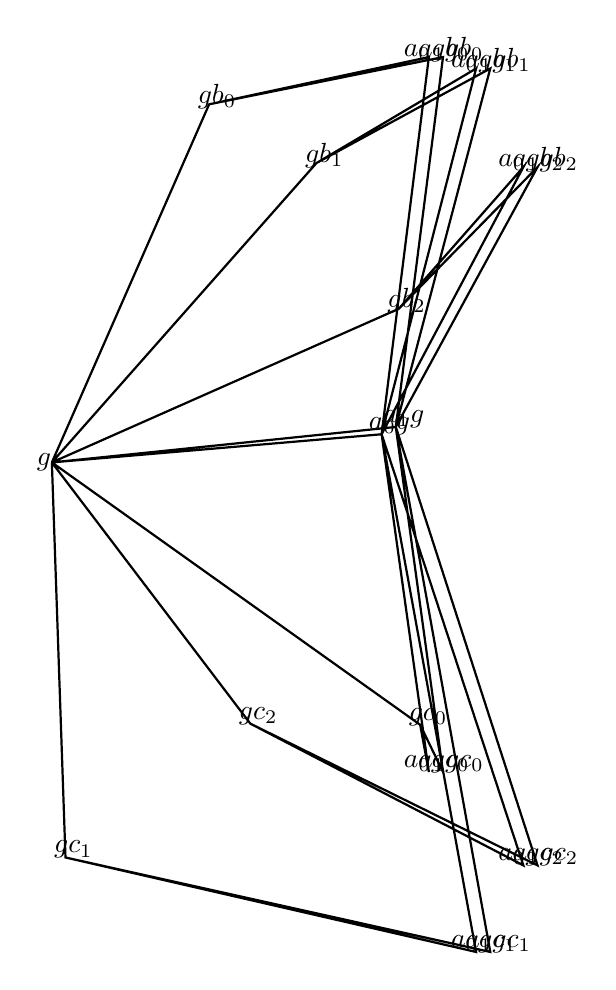
\begin{tikzpicture}
            \draw[thick](0,0)(0,0) -- (1.9972126931202312,4.547937145644979) -- (4.787829056934486,5.1479371456449785) -- (4.187829056934486,0.35766185541834444) -- (0,0)
(0,0) -- (3.3608504014972636,3.802446346694315) -- (5.387829056934486,5.002446346694315) -- (4.187829056934486,0.35766185541834444) -- (0,0)
(0,0) -- (4.405349179033201,1.9509412769499033) -- (5.987829056934486,3.750941276949903) -- (4.187829056934486,0.35766185541834444) -- (0,0)
(0,0) -- (1.9972126931202312,4.547937145644979) -- (4.967628795745843,5.1479371456449785) -- (4.367628795745843,0.45042868165822664) -- (0,0)
(0,0) -- (3.3608504014972636,3.802446346694315) -- (5.5676287957458435,5.002446346694315) -- (4.367628795745843,0.45042868165822664) -- (0,0)
(0,0) -- (4.405349179033201,1.9509412769499033) -- (6.167628795745843,3.750941276949903) -- (4.367628795745843,0.45042868165822664) -- (0,0)
(0,0) -- (4.677479138524687,-3.3324323965399274) -- (4.787829056934486,-3.9324323965399275) -- (4.187829056934486,0.35766185541834444) -- (0,0)
(0,0) -- (0.17285778212342562,-5.017203185367112) -- (5.387829056934486,-6.217203185367112) -- (4.187829056934486,0.35766185541834444) -- (0,0)
(0,0) -- (2.520295363717782,-3.3174860444325462) -- (5.987829056934486,-5.117486044432546) -- (4.187829056934486,0.35766185541834444) -- (0,0)
(0,0) -- (4.677479138524687,-3.3324323965399274) -- (4.967628795745843,-3.9324323965399275) -- (4.367628795745843,0.45042868165822664) -- (0,0)
(0,0) -- (0.17285778212342562,-5.017203185367112) -- (5.5676287957458435,-6.217203185367112) -- (4.367628795745843,0.45042868165822664) -- (0,0)
(0,0) -- (2.520295363717782,-3.3174860444325462) -- (6.167628795745843,-5.117486044432546) -- (4.367628795745843,0.45042868165822664) -- (0,0)
;
\node at (4.8878290569344855,5.247937145644978) {$ a_{ 0  } gb_{ 0 } $};
\node at (5.487829056934486,5.102446346694315) {$ a_{ 0  } gb_{ 1 } $};
\node at (6.087829056934486,3.850941276949903) {$ a_{ 0  } gb_{ 2 } $};
\node at (5.067628795745843,5.247937145644978) {$ a_{ 1  } gb_{ 0 } $};
\node at (5.667628795745843,5.102446346694315) {$ a_{ 1  } gb_{ 1 } $};
\node at (6.267628795745843,3.850941276949903) {$ a_{ 1  } gb_{ 2 } $};
\node at (4.8878290569344855,-3.8324323965399274) {$ a_{ 0  } gc_{ 0 } $};
\node at (5.487829056934486,-6.117203185367113) {$ a_{ 0  } gc_{ 1 } $};
\node at (6.087829056934486,-5.017486044432546) {$ a_{ 0  } gc_{ 2 } $};
\node at (5.067628795745843,-3.8324323965399274) {$ a_{ 1  } gc_{ 0 } $};
\node at (5.667628795745843,-6.117203185367113) {$ a_{ 1  } gc_{ 1 } $};
\node at (6.267628795745843,-5.017486044432546) {$ a_{ 1  } gc_{ 2 } $};
(0,0) -- (4.787829056934486,5.1479371456449785) -- (10.583092131086117,5.747937145644978) -- (9.983092131086117,0.8373941098064694) -- (0,0)
(0,0) -- (5.387829056934486,5.002446346694315) -- (11.183092131086116,6.202446346694315) -- (9.983092131086117,0.8373941098064694) -- (0,0)
(0,0) -- (4.787829056934486,5.1479371456449785) -- (9.917709812587903,5.747937145644978) -- (9.317709812587903,1.5002579284367152) -- (0,0)
(0,0) -- (5.387829056934486,5.002446346694315) -- (10.517709812587903,6.202446346694315) -- (9.317709812587903,1.5002579284367152) -- (0,0)
\node at (-0.1,0) {$ g $};
\node at (4.287829056934486,0.4576618554183445) {$ a_{ 0 }g $};
\node at (4.467628795745843,0.5504286816582267) {$ a_{ 1 }g $};
\node at (2.0972126931202313,4.6479371456449785) {$ gb_{ 0 } $};
\node at (3.4608504014972636,3.902446346694315) {$ gb_{ 1 } $};
\node at (4.5053491790332005,2.0509412769499034) {$ gb_{ 2 } $};
\node at (4.777479138524686,-3.2324323965399273) {$ gc_{ 0 } $};
\node at (0.2728577821234256,-4.9172031853671125) {$ gc_{ 1 } $};
\node at (2.620295363717782,-3.217486044432546) {$ gc_{ 2 } $};

            \end{tikzpicture}
            \end{center}
            \caption{Square of the complex, with edges $(g,ag), (agb, gb) \in E_A,
            (g,gb), (agb, ag) \in E_B.$ \label{fig:square}
            }
            \end{figure}
 \begin{figure}[H]
            %\label{fig:square}
            \begin{center}
            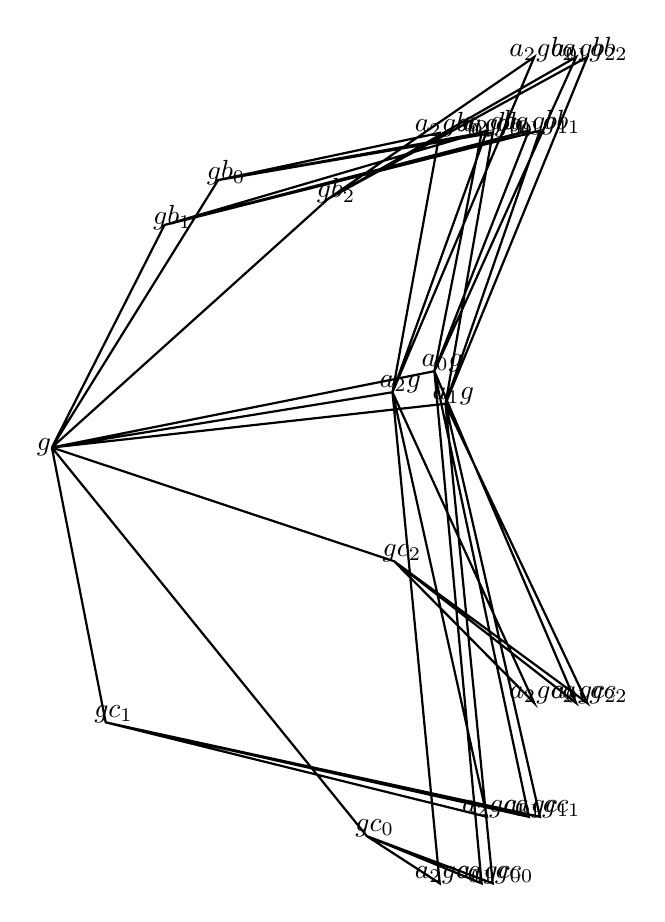
\begin{tikzpicture}
            \draw[thick](0,0)(0,0) -- (2.1122027469037263,3.396414065343364) -- (5.457887752931805,3.996414065343364) -- (4.857887752931806,0.9694613146734061) -- (0,0)
(0,0) -- (1.4301356564336865,2.825341704341864) -- (6.057887752931806,4.025341704341864) -- (4.857887752931806,0.9694613146734061) -- (0,0)
(0,0) -- (3.5100126610879716,3.1586224556540605) -- (6.6578877529318055,4.95862245565406) -- (4.857887752931806,0.9694613146734061) -- (0,0)
(0,0) -- (2.1122027469037263,3.396414065343364) -- (5.598998920801627,3.996414065343364) -- (4.998998920801627,0.555664426941252) -- (0,0)
(0,0) -- (1.4301356564336865,2.825341704341864) -- (6.198998920801627,4.025341704341864) -- (4.998998920801627,0.555664426941252) -- (0,0)
(0,0) -- (3.5100126610879716,3.1586224556540605) -- (6.798998920801627,4.95862245565406) -- (4.998998920801627,0.555664426941252) -- (0,0)
(0,0) -- (2.1122027469037263,3.396414065343364) -- (4.925831752581342,3.996414065343364) -- (4.325831752581342,0.7020195162561511) -- (0,0)
(0,0) -- (1.4301356564336865,2.825341704341864) -- (5.525831752581342,4.025341704341864) -- (4.325831752581342,0.7020195162561511) -- (0,0)
(0,0) -- (3.5100126610879716,3.1586224556540605) -- (6.125831752581342,4.95862245565406) -- (4.325831752581342,0.7020195162561511) -- (0,0)
(0,0) -- (4.000326577625726,-4.935233757781331) -- (5.457887752931805,-5.535233757781331) -- (4.857887752931806,0.9694613146734061) -- (0,0)
(0,0) -- (0.6836998224386526,-3.49032451965724) -- (6.057887752931806,-4.69032451965724) -- (4.857887752931806,0.9694613146734061) -- (0,0)
(0,0) -- (4.346764437824743,-1.444358998934441) -- (6.6578877529318055,-3.244358998934441) -- (4.857887752931806,0.9694613146734061) -- (0,0)
(0,0) -- (4.000326577625726,-4.935233757781331) -- (5.598998920801627,-5.535233757781331) -- (4.998998920801627,0.555664426941252) -- (0,0)
(0,0) -- (0.6836998224386526,-3.49032451965724) -- (6.198998920801627,-4.69032451965724) -- (4.998998920801627,0.555664426941252) -- (0,0)
(0,0) -- (4.346764437824743,-1.444358998934441) -- (6.798998920801627,-3.244358998934441) -- (4.998998920801627,0.555664426941252) -- (0,0)
(0,0) -- (4.000326577625726,-4.935233757781331) -- (4.925831752581342,-5.535233757781331) -- (4.325831752581342,0.7020195162561511) -- (0,0)
(0,0) -- (0.6836998224386526,-3.49032451965724) -- (5.525831752581342,-4.69032451965724) -- (4.325831752581342,0.7020195162561511) -- (0,0)
(0,0) -- (4.346764437824743,-1.444358998934441) -- (6.125831752581342,-3.244358998934441) -- (4.325831752581342,0.7020195162561511) -- (0,0)
;
\node at (5.557887752931805,4.096414065343364) {$ a_{ 0  } gb_{ 0 } $};
\node at (6.1578877529318055,4.125341704341864) {$ a_{ 0  } gb_{ 1 } $};
\node at (6.757887752931805,5.05862245565406) {$ a_{ 0  } gb_{ 2 } $};
\node at (5.6989989208016265,4.096414065343364) {$ a_{ 1  } gb_{ 0 } $};
\node at (6.298998920801627,4.125341704341864) {$ a_{ 1  } gb_{ 1 } $};
\node at (6.898998920801627,5.05862245565406) {$ a_{ 1  } gb_{ 2 } $};
\node at (5.025831752581341,4.096414065343364) {$ a_{ 2  } gb_{ 0 } $};
\node at (5.625831752581342,4.125341704341864) {$ a_{ 2  } gb_{ 1 } $};
\node at (6.225831752581342,5.05862245565406) {$ a_{ 2  } gb_{ 2 } $};
\node at (5.557887752931805,-5.435233757781331) {$ a_{ 0  } gc_{ 0 } $};
\node at (6.1578877529318055,-4.590324519657241) {$ a_{ 0  } gc_{ 1 } $};
\node at (6.757887752931805,-3.144358998934441) {$ a_{ 0  } gc_{ 2 } $};
\node at (5.6989989208016265,-5.435233757781331) {$ a_{ 1  } gc_{ 0 } $};
\node at (6.298998920801627,-4.590324519657241) {$ a_{ 1  } gc_{ 1 } $};
\node at (6.898998920801627,-3.144358998934441) {$ a_{ 1  } gc_{ 2 } $};
\node at (5.025831752581341,-5.435233757781331) {$ a_{ 2  } gc_{ 0 } $};
\node at (5.625831752581342,-4.590324519657241) {$ a_{ 2  } gc_{ 1 } $};
\node at (6.225831752581342,-3.144358998934441) {$ a_{ 2  } gc_{ 2 } $};
(0,0) -- (4.925831752581342,3.996414065343364) -- (10.244058133540628,4.596414065343364) -- (9.644058133540629,1.6870107368654559) -- (0,0)
(0,0) -- (5.525831752581342,4.025341704341864) -- (10.844058133540628,5.225341704341864) -- (9.644058133540629,1.6870107368654559) -- (0,0)
(0,0) -- (6.125831752581342,4.95862245565406) -- (11.44405813354063,6.75862245565406) -- (9.644058133540629,1.6870107368654559) -- (0,0)
(0,0) -- (4.925831752581342,3.996414065343364) -- (10.305902209870363,4.596414065343364) -- (9.705902209870363,1.8360633239775226) -- (0,0)
(0,0) -- (5.525831752581342,4.025341704341864) -- (10.905902209870362,5.225341704341864) -- (9.705902209870363,1.8360633239775226) -- (0,0)
(0,0) -- (6.125831752581342,4.95862245565406) -- (11.505902209870364,6.75862245565406) -- (9.705902209870363,1.8360633239775226) -- (0,0)
(0,0) -- (4.925831752581342,3.996414065343364) -- (10.057512387521948,4.596414065343364) -- (9.457512387521948,1.5581897659196604) -- (0,0)
(0,0) -- (5.525831752581342,4.025341704341864) -- (10.657512387521948,5.225341704341864) -- (9.457512387521948,1.5581897659196604) -- (0,0)
(0,0) -- (6.125831752581342,4.95862245565406) -- (11.257512387521949,6.75862245565406) -- (9.457512387521948,1.5581897659196604) -- (0,0)
\node at (-0.1,0) {$ g $};
\node at (4.957887752931805,1.0694613146734062) {$ a_{ 0 }g $};
\node at (5.098998920801627,0.6556644269412519) {$ a_{ 1 }g $};
\node at (4.425831752581342,0.8020195162561511) {$ a_{ 2 }g $};
\node at (2.2122027469037264,3.496414065343364) {$ gb_{ 0 } $};
\node at (1.5301356564336865,2.925341704341864) {$ gb_{ 1 } $};
\node at (3.6100126610879717,3.2586224556540606) {$ gb_{ 2 } $};
\node at (4.100326577625726,-4.835233757781332) {$ gc_{ 0 } $};
\node at (0.7836998224386525,-3.39032451965724) {$ gc_{ 1 } $};
\node at (4.446764437824743,-1.3443589989344409) {$ gc_{ 2 } $};

            \end{tikzpicture}
            \end{center}
            \caption{Square of the complex, with edges $(g,ag), (agb, gb) \in E_A,
            (g,gb), (agb, ag) \in E_B.$ \label{fig:square}
            }
            \end{figure}
 \begin{figure}[H]
            %\label{fig:square}
            \begin{center}
            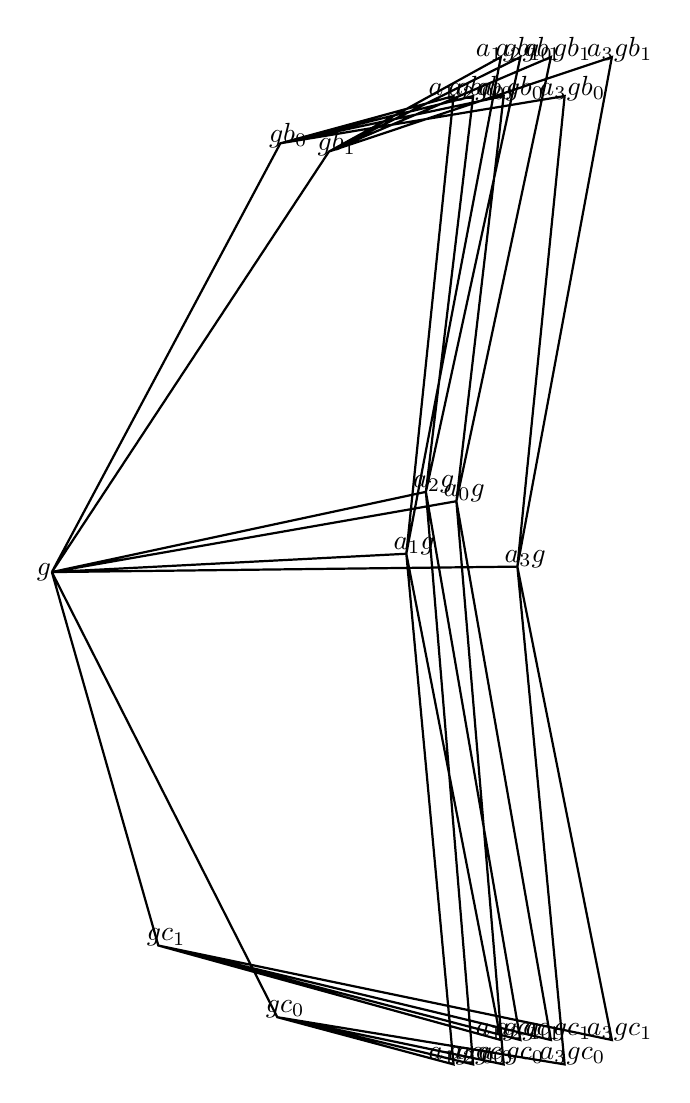
\begin{tikzpicture}
            \draw[thick](0,0)(0,0) -- (2.902132316126874,5.445353809937107) -- (5.737425264333125,6.045353809937106) -- (5.1374252643331255,0.8997822008701404) -- (0,0)
(0,0) -- (3.519261063062803,5.340497599844142) -- (6.337425264333126,6.540497599844143) -- (5.1374252643331255,0.8997822008701404) -- (0,0)
(0,0) -- (2.902132316126874,5.445353809937107) -- (5.101545349270727,6.045353809937106) -- (4.501545349270727,0.23261671756616215) -- (0,0)
(0,0) -- (3.519261063062803,5.340497599844142) -- (5.701545349270727,6.540497599844143) -- (4.501545349270727,0.23261671756616215) -- (0,0)
(0,0) -- (2.902132316126874,5.445353809937107) -- (5.350175674638729,6.045353809937106) -- (4.750175674638729,1.0187007555210184) -- (0,0)
(0,0) -- (3.519261063062803,5.340497599844142) -- (5.9501756746387295,6.540497599844143) -- (4.750175674638729,1.0187007555210184) -- (0,0)
(0,0) -- (2.902132316126874,5.445353809937107) -- (6.511977478861491,6.045353809937106) -- (5.911977478861491,0.06918280102654521) -- (0,0)
(0,0) -- (3.519261063062803,5.340497599844142) -- (7.111977478861491,6.540497599844143) -- (5.911977478861491,0.06918280102654521) -- (0,0)
(0,0) -- (2.8624821157439495,-5.652748904677705) -- (5.737425264333125,-6.252748904677705) -- (5.1374252643331255,0.8997822008701404) -- (0,0)
(0,0) -- (1.3518753975396964,-4.742650949696449) -- (6.337425264333126,-5.942650949696449) -- (5.1374252643331255,0.8997822008701404) -- (0,0)
(0,0) -- (2.8624821157439495,-5.652748904677705) -- (5.101545349270727,-6.252748904677705) -- (4.501545349270727,0.23261671756616215) -- (0,0)
(0,0) -- (1.3518753975396964,-4.742650949696449) -- (5.701545349270727,-5.942650949696449) -- (4.501545349270727,0.23261671756616215) -- (0,0)
(0,0) -- (2.8624821157439495,-5.652748904677705) -- (5.350175674638729,-6.252748904677705) -- (4.750175674638729,1.0187007555210184) -- (0,0)
(0,0) -- (1.3518753975396964,-4.742650949696449) -- (5.9501756746387295,-5.942650949696449) -- (4.750175674638729,1.0187007555210184) -- (0,0)
(0,0) -- (2.8624821157439495,-5.652748904677705) -- (6.511977478861491,-6.252748904677705) -- (5.911977478861491,0.06918280102654521) -- (0,0)
(0,0) -- (1.3518753975396964,-4.742650949696449) -- (7.111977478861491,-5.942650949696449) -- (5.911977478861491,0.06918280102654521) -- (0,0)
;
\node at (5.837425264333125,6.145353809937106) {$ a_{ 0  } gb_{ 0 } $};
\node at (6.437425264333125,6.640497599844142) {$ a_{ 0  } gb_{ 1 } $};
\node at (5.201545349270726,6.145353809937106) {$ a_{ 1  } gb_{ 0 } $};
\node at (5.801545349270727,6.640497599844142) {$ a_{ 1  } gb_{ 1 } $};
\node at (5.450175674638729,6.145353809937106) {$ a_{ 2  } gb_{ 0 } $};
\node at (6.050175674638729,6.640497599844142) {$ a_{ 2  } gb_{ 1 } $};
\node at (6.6119774788614905,6.145353809937106) {$ a_{ 3  } gb_{ 0 } $};
\node at (7.211977478861491,6.640497599844142) {$ a_{ 3  } gb_{ 1 } $};
\node at (5.837425264333125,-6.152748904677705) {$ a_{ 0  } gc_{ 0 } $};
\node at (6.437425264333125,-5.842650949696449) {$ a_{ 0  } gc_{ 1 } $};
\node at (5.201545349270726,-6.152748904677705) {$ a_{ 1  } gc_{ 0 } $};
\node at (5.801545349270727,-5.842650949696449) {$ a_{ 1  } gc_{ 1 } $};
\node at (5.450175674638729,-6.152748904677705) {$ a_{ 2  } gc_{ 0 } $};
\node at (6.050175674638729,-5.842650949696449) {$ a_{ 2  } gc_{ 1 } $};
\node at (6.6119774788614905,-6.152748904677705) {$ a_{ 3  } gc_{ 0 } $};
\node at (7.211977478861491,-5.842650949696449) {$ a_{ 3  } gc_{ 1 } $};
(0,0) -- (5.350175674638729,6.045353809937106) -- (10.026051805316374,6.645353809937106) -- (9.426051805316375,1.4860542116877902) -- (0,0)
(0,0) -- (5.9501756746387295,6.540497599844143) -- (10.626051805316374,7.740497599844143) -- (9.426051805316375,1.4860542116877902) -- (0,0)
(0,0) -- (6.511977478861491,6.045353809937106) -- (11.226051805316374,7.845353809937106) -- (9.426051805316375,1.4860542116877902) -- (0,0)
(0,0) -- (7.111977478861491,6.540497599844143) -- (11.826051805316375,8.940497599844143) -- (9.426051805316375,1.4860542116877902) -- (0,0)
(0,0) -- (5.350175674638729,6.045353809937106) -- (9.74916062573331,6.645353809937106) -- (9.14916062573331,1.6262165700635127) -- (0,0)
(0,0) -- (5.9501756746387295,6.540497599844143) -- (10.34916062573331,7.740497599844143) -- (9.14916062573331,1.6262165700635127) -- (0,0)
(0,0) -- (6.511977478861491,6.045353809937106) -- (10.94916062573331,7.845353809937106) -- (9.14916062573331,1.6262165700635127) -- (0,0)
(0,0) -- (7.111977478861491,6.540497599844143) -- (11.549160625733311,8.940497599844143) -- (9.14916062573331,1.6262165700635127) -- (0,0)
(0,0) -- (5.350175674638729,6.045353809937106) -- (9.412627415869121,6.645353809937106) -- (8.812627415869121,1.7232043246459898) -- (0,0)
(0,0) -- (5.9501756746387295,6.540497599844143) -- (10.01262741586912,7.740497599844143) -- (8.812627415869121,1.7232043246459898) -- (0,0)
(0,0) -- (6.511977478861491,6.045353809937106) -- (10.61262741586912,7.845353809937106) -- (8.812627415869121,1.7232043246459898) -- (0,0)
(0,0) -- (7.111977478861491,6.540497599844143) -- (11.212627415869122,8.940497599844143) -- (8.812627415869121,1.7232043246459898) -- (0,0)
(0,0) -- (5.350175674638729,6.045353809937106) -- (11.33197567643573,6.645353809937106) -- (10.73197567643573,1.8374546598197936) -- (0,0)
(0,0) -- (5.9501756746387295,6.540497599844143) -- (11.93197567643573,7.740497599844143) -- (10.73197567643573,1.8374546598197936) -- (0,0)
(0,0) -- (6.511977478861491,6.045353809937106) -- (12.531975676435732,7.845353809937106) -- (10.73197567643573,1.8374546598197936) -- (0,0)
(0,0) -- (7.111977478861491,6.540497599844143) -- (13.131975676435731,8.940497599844143) -- (10.73197567643573,1.8374546598197936) -- (0,0)
\node at (-0.1,0) {$ g $};
\node at (5.237425264333125,0.9997822008701404) {$ a_{ 0 }g $};
\node at (4.601545349270727,0.3326167175661622) {$ a_{ 1 }g $};
\node at (4.850175674638729,1.1187007555210184) {$ a_{ 2 }g $};
\node at (6.011977478861491,0.1691828010265452) {$ a_{ 3 }g $};
\node at (3.002132316126874,5.545353809937106) {$ gb_{ 0 } $};
\node at (3.6192610630628033,5.440497599844142) {$ gb_{ 1 } $};
\node at (2.9624821157439496,-5.552748904677705) {$ gc_{ 0 } $};
\node at (1.4518753975396965,-4.642650949696449) {$ gc_{ 1 } $};

            \end{tikzpicture}
            \end{center}
            \caption{Square of the complex, with edges $(g,ag), (agb, gb) \in E_A,
            (g,gb), (agb, ag) \in E_B.$ \label{fig:square}
            }
            \end{figure}
 \begin{figure}[H]
            %\label{fig:square}
            \begin{center}
            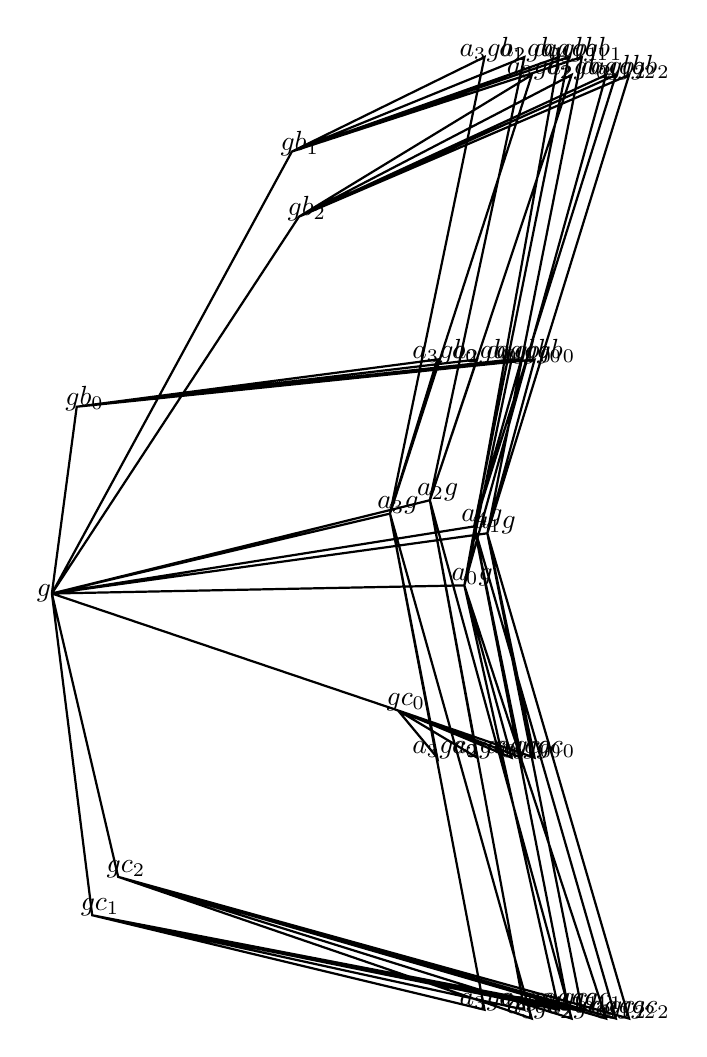
\begin{tikzpicture}
            \draw[thick](0,0)(0,0) -- (0.3157371927488961,2.3718600701120027) -- (5.838319947797693,2.971860070112003) -- (5.238319947797693,0.1031944350387692) -- (0,0)
(0,0) -- (3.0483870159743347,5.612731873988682) -- (6.438319947797694,6.812731873988682) -- (5.238319947797693,0.1031944350387692) -- (0,0)
(0,0) -- (3.1378866292476464,4.785561098190048) -- (7.038319947797693,6.585561098190047) -- (5.238319947797693,0.1031944350387692) -- (0,0)
(0,0) -- (0.3157371927488961,2.3718600701120027) -- (6.1304613837821735,2.971860070112003) -- (5.530461383782174,0.764728711791674) -- (0,0)
(0,0) -- (3.0483870159743347,5.612731873988682) -- (6.730461383782174,6.812731873988682) -- (5.530461383782174,0.764728711791674) -- (0,0)
(0,0) -- (3.1378866292476464,4.785561098190048) -- (7.330461383782174,6.585561098190047) -- (5.530461383782174,0.764728711791674) -- (0,0)
(0,0) -- (0.3157371927488961,2.3718600701120027) -- (5.4002770171072125,2.971860070112003) -- (4.800277017107213,1.1845249636095143) -- (0,0)
(0,0) -- (3.0483870159743347,5.612731873988682) -- (6.000277017107213,6.812731873988682) -- (4.800277017107213,1.1845249636095143) -- (0,0)
(0,0) -- (3.1378866292476464,4.785561098190048) -- (6.600277017107213,6.585561098190047) -- (4.800277017107213,1.1845249636095143) -- (0,0)
(0,0) -- (0.3157371927488961,2.3718600701120027) -- (4.89443958146121,2.971860070112003) -- (4.29443958146121,1.014779549590978) -- (0,0)
(0,0) -- (3.0483870159743347,5.612731873988682) -- (5.494439581461211,6.812731873988682) -- (4.29443958146121,1.014779549590978) -- (0,0)
(0,0) -- (3.1378866292476464,4.785561098190048) -- (6.09443958146121,6.585561098190047) -- (4.29443958146121,1.014779549590978) -- (0,0)
(0,0) -- (0.3157371927488961,2.3718600701120027) -- (5.9626796708559615,2.971860070112003) -- (5.362679670855962,0.8521411769007804) -- (0,0)
(0,0) -- (3.0483870159743347,5.612731873988682) -- (6.562679670855962,6.812731873988682) -- (5.362679670855962,0.8521411769007804) -- (0,0)
(0,0) -- (3.1378866292476464,4.785561098190048) -- (7.162679670855962,6.585561098190047) -- (5.362679670855962,0.8521411769007804) -- (0,0)
(0,0) -- (4.395605078908026,-1.4847776888122106) -- (5.838319947797693,-2.0847776888122107) -- (5.238319947797693,0.1031944350387692) -- (0,0)
(0,0) -- (0.5123469305985201,-4.085913873455456) -- (6.438319947797694,-5.285913873455456) -- (5.238319947797693,0.1031944350387692) -- (0,0)
(0,0) -- (0.8419002981713164,-3.5980545430063495) -- (7.038319947797693,-5.398054543006349) -- (5.238319947797693,0.1031944350387692) -- (0,0)
(0,0) -- (4.395605078908026,-1.4847776888122106) -- (6.1304613837821735,-2.0847776888122107) -- (5.530461383782174,0.764728711791674) -- (0,0)
(0,0) -- (0.5123469305985201,-4.085913873455456) -- (6.730461383782174,-5.285913873455456) -- (5.530461383782174,0.764728711791674) -- (0,0)
(0,0) -- (0.8419002981713164,-3.5980545430063495) -- (7.330461383782174,-5.398054543006349) -- (5.530461383782174,0.764728711791674) -- (0,0)
(0,0) -- (4.395605078908026,-1.4847776888122106) -- (5.4002770171072125,-2.0847776888122107) -- (4.800277017107213,1.1845249636095143) -- (0,0)
(0,0) -- (0.5123469305985201,-4.085913873455456) -- (6.000277017107213,-5.285913873455456) -- (4.800277017107213,1.1845249636095143) -- (0,0)
(0,0) -- (0.8419002981713164,-3.5980545430063495) -- (6.600277017107213,-5.398054543006349) -- (4.800277017107213,1.1845249636095143) -- (0,0)
(0,0) -- (4.395605078908026,-1.4847776888122106) -- (4.89443958146121,-2.0847776888122107) -- (4.29443958146121,1.014779549590978) -- (0,0)
(0,0) -- (0.5123469305985201,-4.085913873455456) -- (5.494439581461211,-5.285913873455456) -- (4.29443958146121,1.014779549590978) -- (0,0)
(0,0) -- (0.8419002981713164,-3.5980545430063495) -- (6.09443958146121,-5.398054543006349) -- (4.29443958146121,1.014779549590978) -- (0,0)
(0,0) -- (4.395605078908026,-1.4847776888122106) -- (5.9626796708559615,-2.0847776888122107) -- (5.362679670855962,0.8521411769007804) -- (0,0)
(0,0) -- (0.5123469305985201,-4.085913873455456) -- (6.562679670855962,-5.285913873455456) -- (5.362679670855962,0.8521411769007804) -- (0,0)
(0,0) -- (0.8419002981713164,-3.5980545430063495) -- (7.162679670855962,-5.398054543006349) -- (5.362679670855962,0.8521411769007804) -- (0,0)
;
\node at (5.938319947797693,3.071860070112003) {$ a_{ 0  } gb_{ 0 } $};
\node at (6.538319947797693,6.912731873988681) {$ a_{ 0  } gb_{ 1 } $};
\node at (7.138319947797693,6.685561098190047) {$ a_{ 0  } gb_{ 2 } $};
\node at (6.230461383782173,3.071860070112003) {$ a_{ 1  } gb_{ 0 } $};
\node at (6.830461383782174,6.912731873988681) {$ a_{ 1  } gb_{ 1 } $};
\node at (7.430461383782173,6.685561098190047) {$ a_{ 1  } gb_{ 2 } $};
\node at (5.500277017107212,3.071860070112003) {$ a_{ 2  } gb_{ 0 } $};
\node at (6.100277017107213,6.912731873988681) {$ a_{ 2  } gb_{ 1 } $};
\node at (6.700277017107212,6.685561098190047) {$ a_{ 2  } gb_{ 2 } $};
\node at (4.99443958146121,3.071860070112003) {$ a_{ 3  } gb_{ 0 } $};
\node at (5.59443958146121,6.912731873988681) {$ a_{ 3  } gb_{ 1 } $};
\node at (6.19443958146121,6.685561098190047) {$ a_{ 3  } gb_{ 2 } $};
\node at (6.062679670855961,3.071860070112003) {$ a_{ 4  } gb_{ 0 } $};
\node at (6.662679670855962,6.912731873988681) {$ a_{ 4  } gb_{ 1 } $};
\node at (7.262679670855961,6.685561098190047) {$ a_{ 4  } gb_{ 2 } $};
\node at (5.938319947797693,-1.9847776888122106) {$ a_{ 0  } gc_{ 0 } $};
\node at (6.538319947797693,-5.185913873455457) {$ a_{ 0  } gc_{ 1 } $};
\node at (7.138319947797693,-5.29805454300635) {$ a_{ 0  } gc_{ 2 } $};
\node at (6.230461383782173,-1.9847776888122106) {$ a_{ 1  } gc_{ 0 } $};
\node at (6.830461383782174,-5.185913873455457) {$ a_{ 1  } gc_{ 1 } $};
\node at (7.430461383782173,-5.29805454300635) {$ a_{ 1  } gc_{ 2 } $};
\node at (5.500277017107212,-1.9847776888122106) {$ a_{ 2  } gc_{ 0 } $};
\node at (6.100277017107213,-5.185913873455457) {$ a_{ 2  } gc_{ 1 } $};
\node at (6.700277017107212,-5.29805454300635) {$ a_{ 2  } gc_{ 2 } $};
\node at (4.99443958146121,-1.9847776888122106) {$ a_{ 3  } gc_{ 0 } $};
\node at (5.59443958146121,-5.185913873455457) {$ a_{ 3  } gc_{ 1 } $};
\node at (6.19443958146121,-5.29805454300635) {$ a_{ 3  } gc_{ 2 } $};
\node at (6.062679670855961,-1.9847776888122106) {$ a_{ 4  } gc_{ 0 } $};
\node at (6.662679670855962,-5.185913873455457) {$ a_{ 4  } gc_{ 1 } $};
\node at (7.262679670855961,-5.29805454300635) {$ a_{ 4  } gc_{ 2 } $};
(0,0) -- (5.9626796708559615,2.971860070112003) -- (10.275615637012875,3.571860070112003) -- (9.675615637012875,1.311587489197739) -- (0,0)
(0,0) -- (6.562679670855962,6.812731873988682) -- (10.875615637012874,8.012731873988681) -- (9.675615637012875,1.311587489197739) -- (0,0)
(0,0) -- (7.162679670855962,6.585561098190047) -- (11.475615637012876,8.385561098190047) -- (9.675615637012875,1.311587489197739) -- (0,0)
(0,0) -- (5.9626796708559615,2.971860070112003) -- (10.466588148519195,3.571860070112003) -- (9.866588148519195,1.1738867716137373) -- (0,0)
(0,0) -- (6.562679670855962,6.812731873988682) -- (11.066588148519195,8.012731873988681) -- (9.866588148519195,1.1738867716137373) -- (0,0)
(0,0) -- (7.162679670855962,6.585561098190047) -- (11.666588148519196,8.385561098190047) -- (9.866588148519195,1.1738867716137373) -- (0,0)
(0,0) -- (5.9626796708559615,2.971860070112003) -- (11.490491771753629,3.571860070112003) -- (10.890491771753629,0.9810510721823535) -- (0,0)
(0,0) -- (6.562679670855962,6.812731873988682) -- (12.090491771753628,8.012731873988681) -- (10.890491771753629,0.9810510721823535) -- (0,0)
(0,0) -- (7.162679670855962,6.585561098190047) -- (12.690491771753628,8.385561098190047) -- (10.890491771753629,0.9810510721823535) -- (0,0)
(0,0) -- (5.9626796708559615,2.971860070112003) -- (11.81137114149538,3.571860070112003) -- (11.21137114149538,1.6101636795300696) -- (0,0)
(0,0) -- (6.562679670855962,6.812731873988682) -- (12.41137114149538,8.012731873988681) -- (11.21137114149538,1.6101636795300696) -- (0,0)
(0,0) -- (7.162679670855962,6.585561098190047) -- (13.011371141495381,8.385561098190047) -- (11.21137114149538,1.6101636795300696) -- (0,0)
(0,0) -- (5.9626796708559615,2.971860070112003) -- (11.114988109440917,3.571860070112003) -- (10.514988109440917,1.7637601984769191) -- (0,0)
(0,0) -- (6.562679670855962,6.812731873988682) -- (11.714988109440917,8.012731873988681) -- (10.514988109440917,1.7637601984769191) -- (0,0)
(0,0) -- (7.162679670855962,6.585561098190047) -- (12.314988109440918,8.385561098190047) -- (10.514988109440917,1.7637601984769191) -- (0,0)
\node at (-0.1,0) {$ g $};
\node at (5.338319947797693,0.20319443503876922) {$ a_{ 0 }g $};
\node at (5.6304613837821735,0.864728711791674) {$ a_{ 1 }g $};
\node at (4.9002770171072125,1.2845249636095144) {$ a_{ 2 }g $};
\node at (4.39443958146121,1.114779549590978) {$ a_{ 3 }g $};
\node at (5.4626796708559615,0.9521411769007804) {$ a_{ 4 }g $};
\node at (0.4157371927488961,2.471860070112003) {$ gb_{ 0 } $};
\node at (3.148387015974335,5.712731873988681) {$ gb_{ 1 } $};
\node at (3.2378866292476465,4.885561098190047) {$ gb_{ 2 } $};
\node at (4.495605078908025,-1.3847776888122105) {$ gc_{ 0 } $};
\node at (0.6123469305985201,-3.985913873455456) {$ gc_{ 1 } $};
\node at (0.9419002981713164,-3.4980545430063494) {$ gc_{ 2 } $};

            \end{tikzpicture}
            \end{center}
            \caption{Square of the complex, with edges $(g,ag), (agb, gb) \in E_A,
            (g,gb), (agb, ag) \in E_B.$ \label{fig:square}
            }
            \end{figure}
 \begin{figure}[H]
            %\label{fig:square}
            \begin{center}
            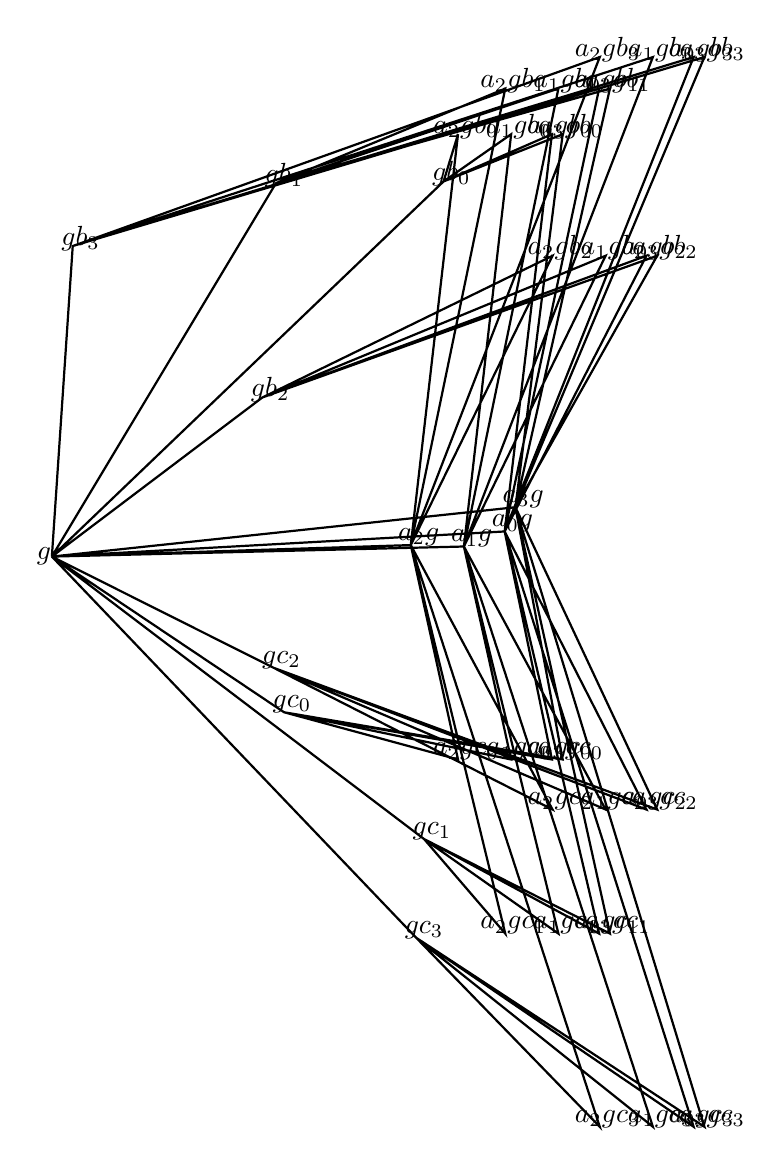
\begin{tikzpicture}
            \draw[thick](0,0)(0,0) -- (4.974303594853455,4.763666170248685) -- (6.350421920034709,5.363666170248685) -- (5.750421920034709,0.31882236115696105) -- (0,0)
(0,0) -- (2.847137724288113,4.743408733945191) -- (6.950421920034709,5.9434087339451915) -- (5.750421920034709,0.31882236115696105) -- (0,0)
(0,0) -- (2.672978287320281,2.0201649283974046) -- (7.550421920034709,3.8201649283974044) -- (5.750421920034709,0.31882236115696105) -- (0,0)
(0,0) -- (0.2650185101889735,3.9436376962397848) -- (8.15042192003471,6.343637696239785) -- (5.750421920034709,0.31882236115696105) -- (0,0)
(0,0) -- (4.974303594853455,4.763666170248685) -- (5.8327832748062445,5.363666170248685) -- (5.232783274806245,0.1277270333944404) -- (0,0)
(0,0) -- (2.847137724288113,4.743408733945191) -- (6.432783274806245,5.9434087339451915) -- (5.232783274806245,0.1277270333944404) -- (0,0)
(0,0) -- (2.672978287320281,2.0201649283974046) -- (7.032783274806245,3.8201649283974044) -- (5.232783274806245,0.1277270333944404) -- (0,0)
(0,0) -- (0.2650185101889735,3.9436376962397848) -- (7.632783274806245,6.343637696239785) -- (5.232783274806245,0.1277270333944404) -- (0,0)
(0,0) -- (4.974303594853455,4.763666170248685) -- (5.1581077730514275,5.363666170248685) -- (4.558107773051428,0.14594331632203422) -- (0,0)
(0,0) -- (2.847137724288113,4.743408733945191) -- (5.758107773051428,5.9434087339451915) -- (4.558107773051428,0.14594331632203422) -- (0,0)
(0,0) -- (2.672978287320281,2.0201649283974046) -- (6.358107773051428,3.8201649283974044) -- (4.558107773051428,0.14594331632203422) -- (0,0)
(0,0) -- (0.2650185101889735,3.9436376962397848) -- (6.958107773051427,6.343637696239785) -- (4.558107773051428,0.14594331632203422) -- (0,0)
(0,0) -- (4.974303594853455,4.763666170248685) -- (6.487216679058061,5.363666170248685) -- (5.887216679058062,0.6264036594607362) -- (0,0)
(0,0) -- (2.847137724288113,4.743408733945191) -- (7.087216679058062,5.9434087339451915) -- (5.887216679058062,0.6264036594607362) -- (0,0)
(0,0) -- (2.672978287320281,2.0201649283974046) -- (7.687216679058062,3.8201649283974044) -- (5.887216679058062,0.6264036594607362) -- (0,0)
(0,0) -- (0.2650185101889735,3.9436376962397848) -- (8.287216679058062,6.343637696239785) -- (5.887216679058062,0.6264036594607362) -- (0,0)
(0,0) -- (2.9481382176131765,-1.9770285063278377) -- (6.350421920034709,-2.5770285063278378) -- (5.750421920034709,0.31882236115696105) -- (0,0)
(0,0) -- (4.727665514602651,-3.588171128387879) -- (6.950421920034709,-4.788171128387879) -- (5.750421920034709,0.31882236115696105) -- (0,0)
(0,0) -- (2.8154385111180957,-1.412218847268004) -- (7.550421920034709,-3.2122188472680038) -- (5.750421920034709,0.31882236115696105) -- (0,0)
(0,0) -- (4.627132493472391,-4.8413148873213565) -- (8.15042192003471,-7.241314887321357) -- (5.750421920034709,0.31882236115696105) -- (0,0)
(0,0) -- (2.9481382176131765,-1.9770285063278377) -- (5.8327832748062445,-2.5770285063278378) -- (5.232783274806245,0.1277270333944404) -- (0,0)
(0,0) -- (4.727665514602651,-3.588171128387879) -- (6.432783274806245,-4.788171128387879) -- (5.232783274806245,0.1277270333944404) -- (0,0)
(0,0) -- (2.8154385111180957,-1.412218847268004) -- (7.032783274806245,-3.2122188472680038) -- (5.232783274806245,0.1277270333944404) -- (0,0)
(0,0) -- (4.627132493472391,-4.8413148873213565) -- (7.632783274806245,-7.241314887321357) -- (5.232783274806245,0.1277270333944404) -- (0,0)
(0,0) -- (2.9481382176131765,-1.9770285063278377) -- (5.1581077730514275,-2.5770285063278378) -- (4.558107773051428,0.14594331632203422) -- (0,0)
(0,0) -- (4.727665514602651,-3.588171128387879) -- (5.758107773051428,-4.788171128387879) -- (4.558107773051428,0.14594331632203422) -- (0,0)
(0,0) -- (2.8154385111180957,-1.412218847268004) -- (6.358107773051428,-3.2122188472680038) -- (4.558107773051428,0.14594331632203422) -- (0,0)
(0,0) -- (4.627132493472391,-4.8413148873213565) -- (6.958107773051427,-7.241314887321357) -- (4.558107773051428,0.14594331632203422) -- (0,0)
(0,0) -- (2.9481382176131765,-1.9770285063278377) -- (6.487216679058061,-2.5770285063278378) -- (5.887216679058062,0.6264036594607362) -- (0,0)
(0,0) -- (4.727665514602651,-3.588171128387879) -- (7.087216679058062,-4.788171128387879) -- (5.887216679058062,0.6264036594607362) -- (0,0)
(0,0) -- (2.8154385111180957,-1.412218847268004) -- (7.687216679058062,-3.2122188472680038) -- (5.887216679058062,0.6264036594607362) -- (0,0)
(0,0) -- (4.627132493472391,-4.8413148873213565) -- (8.287216679058062,-7.241314887321357) -- (5.887216679058062,0.6264036594607362) -- (0,0)
;
\node at (6.450421920034708,5.463666170248684) {$ a_{ 0  } gb_{ 0 } $};
\node at (7.050421920034709,6.043408733945191) {$ a_{ 0  } gb_{ 1 } $};
\node at (7.650421920034709,3.9201649283974045) {$ a_{ 0  } gb_{ 2 } $};
\node at (8.250421920034709,6.443637696239785) {$ a_{ 0  } gb_{ 3 } $};
\node at (5.932783274806244,5.463666170248684) {$ a_{ 1  } gb_{ 0 } $};
\node at (6.532783274806245,6.043408733945191) {$ a_{ 1  } gb_{ 1 } $};
\node at (7.132783274806244,3.9201649283974045) {$ a_{ 1  } gb_{ 2 } $};
\node at (7.732783274806245,6.443637696239785) {$ a_{ 1  } gb_{ 3 } $};
\node at (5.258107773051427,5.463666170248684) {$ a_{ 2  } gb_{ 0 } $};
\node at (5.858107773051428,6.043408733945191) {$ a_{ 2  } gb_{ 1 } $};
\node at (6.458107773051427,3.9201649283974045) {$ a_{ 2  } gb_{ 2 } $};
\node at (7.058107773051427,6.443637696239785) {$ a_{ 2  } gb_{ 3 } $};
\node at (6.587216679058061,5.463666170248684) {$ a_{ 3  } gb_{ 0 } $};
\node at (7.187216679058062,6.043408733945191) {$ a_{ 3  } gb_{ 1 } $};
\node at (7.787216679058061,3.9201649283974045) {$ a_{ 3  } gb_{ 2 } $};
\node at (8.387216679058062,6.443637696239785) {$ a_{ 3  } gb_{ 3 } $};
\node at (6.450421920034708,-2.4770285063278377) {$ a_{ 0  } gc_{ 0 } $};
\node at (7.050421920034709,-4.6881711283878795) {$ a_{ 0  } gc_{ 1 } $};
\node at (7.650421920034709,-3.1122188472680037) {$ a_{ 0  } gc_{ 2 } $};
\node at (8.250421920034709,-7.141314887321357) {$ a_{ 0  } gc_{ 3 } $};
\node at (5.932783274806244,-2.4770285063278377) {$ a_{ 1  } gc_{ 0 } $};
\node at (6.532783274806245,-4.6881711283878795) {$ a_{ 1  } gc_{ 1 } $};
\node at (7.132783274806244,-3.1122188472680037) {$ a_{ 1  } gc_{ 2 } $};
\node at (7.732783274806245,-7.141314887321357) {$ a_{ 1  } gc_{ 3 } $};
\node at (5.258107773051427,-2.4770285063278377) {$ a_{ 2  } gc_{ 0 } $};
\node at (5.858107773051428,-4.6881711283878795) {$ a_{ 2  } gc_{ 1 } $};
\node at (6.458107773051427,-3.1122188472680037) {$ a_{ 2  } gc_{ 2 } $};
\node at (7.058107773051427,-7.141314887321357) {$ a_{ 2  } gc_{ 3 } $};
\node at (6.587216679058061,-2.4770285063278377) {$ a_{ 3  } gc_{ 0 } $};
\node at (7.187216679058062,-4.6881711283878795) {$ a_{ 3  } gc_{ 1 } $};
\node at (7.787216679058061,-3.1122188472680037) {$ a_{ 3  } gc_{ 2 } $};
\node at (8.387216679058062,-7.141314887321357) {$ a_{ 3  } gc_{ 3 } $};
(0,0) -- (5.8327832748062445,5.363666170248685) -- (10.579609129049212,5.963666170248684) -- (9.979609129049212,0.5689114938244543) -- (0,0)
(0,0) -- (6.432783274806245,5.9434087339451915) -- (11.179609129049211,7.143408733945192) -- (9.979609129049212,0.5689114938244543) -- (0,0)
(0,0) -- (7.032783274806245,3.8201649283974044) -- (11.779609129049213,5.620164928397404) -- (9.979609129049212,0.5689114938244543) -- (0,0)
(0,0) -- (7.632783274806245,6.343637696239785) -- (12.379609129049213,8.743637696239785) -- (9.979609129049212,0.5689114938244543) -- (0,0)
(0,0) -- (5.8327832748062445,5.363666170248685) -- (10.882314285430175,5.963666170248684) -- (10.282314285430175,1.0267463091673366) -- (0,0)
(0,0) -- (6.432783274806245,5.9434087339451915) -- (11.482314285430174,7.143408733945192) -- (10.282314285430175,1.0267463091673366) -- (0,0)
(0,0) -- (7.032783274806245,3.8201649283974044) -- (12.082314285430176,5.620164928397404) -- (10.282314285430175,1.0267463091673366) -- (0,0)
(0,0) -- (7.632783274806245,6.343637696239785) -- (12.682314285430175,8.743637696239785) -- (10.282314285430175,1.0267463091673366) -- (0,0)
(0,0) -- (5.8327832748062445,5.363666170248685) -- (11.61636146332181,5.963666170248684) -- (11.016361463321811,1.2774610460108975) -- (0,0)
(0,0) -- (6.432783274806245,5.9434087339451915) -- (12.21636146332181,7.143408733945192) -- (11.016361463321811,1.2774610460108975) -- (0,0)
(0,0) -- (7.032783274806245,3.8201649283974044) -- (12.816361463321812,5.620164928397404) -- (11.016361463321811,1.2774610460108975) -- (0,0)
(0,0) -- (7.632783274806245,6.343637696239785) -- (13.416361463321811,8.743637696239785) -- (11.016361463321811,1.2774610460108975) -- (0,0)
(0,0) -- (5.8327832748062445,5.363666170248685) -- (10.127975627326107,5.963666170248684) -- (9.527975627326107,0.8466547852721737) -- (0,0)
(0,0) -- (6.432783274806245,5.9434087339451915) -- (10.727975627326106,7.143408733945192) -- (9.527975627326107,0.8466547852721737) -- (0,0)
(0,0) -- (7.032783274806245,3.8201649283974044) -- (11.327975627326108,5.620164928397404) -- (9.527975627326107,0.8466547852721737) -- (0,0)
(0,0) -- (7.632783274806245,6.343637696239785) -- (11.927975627326107,8.743637696239785) -- (9.527975627326107,0.8466547852721737) -- (0,0)
\node at (-0.1,0) {$ g $};
\node at (5.850421920034709,0.41882236115696103) {$ a_{ 0 }g $};
\node at (5.3327832748062445,0.2277270333944404) {$ a_{ 1 }g $};
\node at (4.6581077730514275,0.24594331632203423) {$ a_{ 2 }g $};
\node at (5.987216679058061,0.7264036594607362) {$ a_{ 3 }g $};
\node at (5.074303594853455,4.863666170248685) {$ gb_{ 0 } $};
\node at (2.947137724288113,4.843408733945191) {$ gb_{ 1 } $};
\node at (2.772978287320281,2.1201649283974047) {$ gb_{ 2 } $};
\node at (0.36501851018897347,4.043637696239784) {$ gb_{ 3 } $};
\node at (3.0481382176131766,-1.8770285063278376) {$ gc_{ 0 } $};
\node at (4.827665514602651,-3.488171128387879) {$ gc_{ 1 } $};
\node at (2.915438511118096,-1.3122188472680039) {$ gc_{ 2 } $};
\node at (4.727132493472391,-4.741314887321357) {$ gc_{ 3 } $};

            \end{tikzpicture}
            \end{center}
            \caption{Square of the complex, with edges $(g,ag), (agb, gb) \in E_A,
            (g,gb), (agb, ag) \in E_B.$ \label{fig:square}
            }
            \end{figure}
 
%\end{multicols*}
  % \printbibliography 
\end{document}

 